\begin{exercise}{%
    Határozzuk meg az alábbi integrál értékét a $(0;0)$, $(2,0)$, $(2;2)$
    csúcspontokkal rendelkező, háromszög alapú tartományon!
  }
  \[
    \int_A 8xy \, \mathrm dA
  \]

  \exsol[3cm]{%
    \begin{minipage}[t]{6.5cm}
      A tartomány szemléltetése:
      \begin{center}
        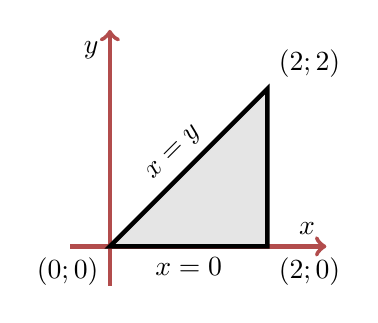
\begin{tikzpicture}[thick]
          \draw[-to, draw=red!40!gray, ultra thick]
          (-0.5, 0) -- (2.75, 0) node[above left] {$x$};
          \draw[-to, draw=red!40!gray, ultra thick]
          (0, -0.5) -- (0, 2.75) node[below left] {$y$};

          \draw[
            ultra thick,
             fill = gray!20,
          ] (0,0) node[below left] {$(0;0)$}
          -- (2,0) node[below right] {$(2;0)$} node[midway, below] {$x = 0$}
          -- (2,2) node[above right] {$(2;2)$}
          -- cycle node[midway,above,rotate=45] {$x = y$}
          ;
        \end{tikzpicture}
      \end{center}
    \end{minipage}%
    \hfill%
    \begin{minipage}[t]{7.5cm}
      A tartomány felírása:
      \vspace{12mm}
      \[
        T = \Big\{\;
        (x;y) \;\Big|\Big.\; 0 < x < y \;\land\; 0 < y < 2
        \;\Big\}
        \text.
      \]
    \end{minipage}%
    \hfill%

    \vspace{5mm}
    Végezzük el az integrálást:
    \[
      \int_0^2 \int_0^y 8xy \, \mathrm dx \, \mathrm dy =
      \int_0^2  \Big[ 4x^2y  \Big]_0^y \, \mathrm dy =
      \int_0^3  4y^3 \, \mathrm dy =
      \Big[ y^4 \Big]_0^2 =
      2^4 - 0^4 =
      16
      \text.
    \]
  }
\end{exercise}
